% A simple cycle
% Author : Jerome Tremblay
\documentclass{article}
\usepackage{tikz}
\begin{document}
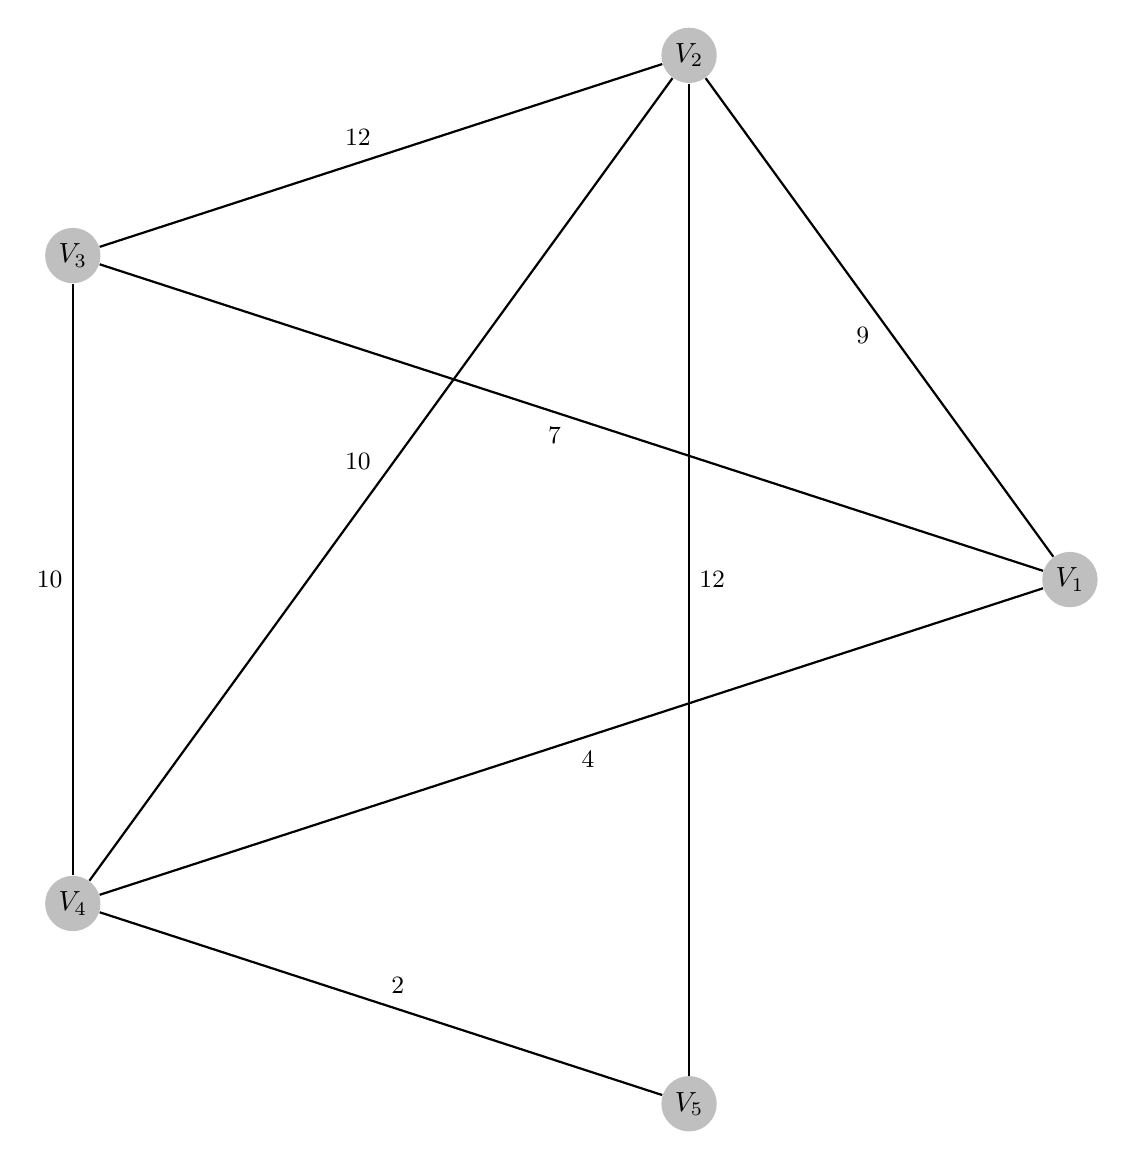
\begin{tikzpicture}[auto]

\tikzstyle{vertex}=[circle,fill=black!25,minimum size=20pt,inner sep=0pt]
\tikzstyle{edge} = [draw,thick,-]
\tikzstyle{weight} = [font=\small]

\def \n {5}
\def \radius {7cm}

\foreach \s in {1,...,\n}
{
  \node[vertex] (\s) at ({360/\n * (\s-1 )}:\radius) {$V_{\s}$};
}

 \foreach \source/ \dest /\weight in {1/2/9, 1/3/7, 1/4/4, 2/5/12, 3/2/12, 4/3/10, 4/2/10, 4/5/2}
{
   \path[edge] (\source) -- node[weight] {$\weight$} (\dest);
}
\end{tikzpicture}
\end{document}